\chapter{Preliminares}
\label{sec:preliminares}

Este capítulo establece los fundamentos teóricos necesarios para abordar el problema de descubrir expresiones analíticas de los ceros de sistemas de ecuaciones no lineales mediante regresión simbólica. En la primera parte (\ref{sec:sistemas}) se introduce la notación y las propiedades de los sistemas de ecuaciones no lineales paramétricos, destacando la multiplicidad de soluciones que pueden existir para una misma tupla de parámetros; se describen los métodos numéricos para el cálculo de ceros de tales sistemas, tanto los métodos iterativos clásicos como el método híbrido de Powell implementado en la biblioteca \texttt{SciPy} \cite{virtanen2020scipy}, y se definen formalmente los conceptos de distancia euclidiana y producto cartesiano, que serán utilizados en la generación del conjunto de datos de entrenamiento. Posteriormente, en la sección \ref{sec:regresion} se abordan los principios de la regresión simbólica \cite{koza1992genetic}, una técnica de aprendizaje automático que permite inferir expresiones algebraicas a partir de datos, y se explican los fundamentos de la programación genética, las funciones de pérdida que guían el proceso evolutivo y los parámetros que controlan el comportamiento del algoritmo. Por último, se presentan los fundamentos de la prueba t de Student para muestras pareadas, que se empleará en el capítulo de experimentación para comparar estadísticamente las distintas configuraciones del algoritmo.

\section{Sistemas de ecuaciones no lineales paramétricos}
\label{sec:sistemas}

En esta sección se formaliza el concepto de sistema de ecuaciones no lineales dependiente de parámetros, así como las herramientas numéricas y matemáticas necesarias para su estudio.

Un sistema de ecuaciones no lineales paramétrico se expresa como la búsqueda de vectores \(\xvec \in \R^n\) que satisfacen
\begin{equation}
\Fvec(\xvec; \thetavec) = \mathbf{0}, \label{eq:sistema_general}
\end{equation}
donde:
\begin{itemize}
    \item \(\Fvec: \R^n \times \R^p \to \R^n\) es una función vectorial no lineal,
    \item \(\xvec = (x_1, \dots, x_n)^T \in \R^n\) es el vector de variables incógnita,
    \item \(\thetavec = (\theta_1, \dots, \theta_p)^T \in \R^p\) es el vector de parámetros del modelo,
    \item \(\mathbf{0} \in \R^n\) denota el vector nulo.
\end{itemize}
La notación \(\Fvec(\xvec; \thetavec)\) indica que \(\Fvec\) depende explícitamente de las variables \(\xvec\) y de los parámetros
\(\thetavec\), estos últimos se consideran fijos durante el proceso de
resolución del sistema de ecuaciones.

\noindent\textbf{Ejemplo 1.} Considérese el sistema de dos ecuaciones
\[
\Fvec(\xvec; \thetavec) =
\begin{pmatrix}
(x_1 - a)(x_2 - ab) \\[2pt] x_1 x_2 - a b^2
\end{pmatrix}
= \mathbf{0},
\]
con \(\xvec = (x_1, x_2)^T \in \R^2\) y parámetros
\(\thetavec = (a, b)^T\), \(a > 0\), \(b > 0\).

Este sistema posee dos soluciones reales para cada tupla de parámetros: \(\xvec = (a, b^2)\) y \(\xvec = (b, ab)\). Nótese que la primera componente de la solución \((a, b^2)\) anula el factor
\((x_1 - a)\) de la primera ecuación, mientras que en la solución
\((b, ab)\) es la segunda componente la que anula el factor
\((x_2 - ab)\). Esta multiplicidad de ceros y su dependencia explícita
de los parámetros ilustran el tipo de fenómenos que aparecen en sistemas no lineales paramétricos y motivan la necesidad de determinar, para cada valor de los parámetros, todas las raíces que serán utilizadas en la construcción del conjunto de datos de entrenamiento con el que se alimentará la regresión simbólica.

La no linealidad de \(\Fvec\) implica que, a diferencia de los sistemas lineales, no existe un método directo general para obtener todas las soluciones, y la estructura del conjunto solución puede ser compleja. Por esta razón se recurre a métodos numéricos iterativos, que se describen en la siguiente sección.

\subsection{Métodos numéricos para el cálculo de ceros}

Una vez definido el sistema no lineal paramétrico, es necesario obtener numéricamente sus soluciones para distintas tuplas de parámetros. Dado que, salvo en casos triviales, no es posible despejar analíticamente las raíces de un sistema no lineal arbitrario, se recurre a métodos iterativos que aproximan las soluciones de manera sucesiva. A continuación se describen dos de los métodos más utilizados, que serán empleados en la etapa de generación de datos, es decir, en la construcción del conjunto de entrenamiento que alimentará la regresión simbólica.

Para sistemas no lineales generales, la obtención de soluciones explícitas mediante métodos simbólicos no es factible, ya que la mayoría de estos sistemas carecen de soluciones expresables en forma cerrada \cite{burden2010numerical}. En su lugar, se emplean métodos numéricos iterativos que, partiendo de una aproximación inicial \(\xvec^{(0)}\), generan una sucesión \(\{\xvec^{(k)}\}_{k=0}^{\infty}\) que converge a una solución \(\xvec^*\), siempre que la aproximación inicial esté suficientemente cerca de dicha solución y que \(\Fvec\) sea diferenciable con jacobiano no singular en \(\xvec^*\) \cite{nocedal2006numerical}.

El método de Newton-Raphson para sistemas no lineales \cite{burden2010numerical} se define mediante la iteración
\begin{equation}
\xvec^{(k+1)} = \xvec^{(k)} - \bigl[\jac_{\Fvec}(\xvec^{(k)})\bigr]^{-1} \Fvec(\xvec^{(k)}; \thetavec), \label{eq:newton}
\end{equation}
donde:
\begin{itemize}
    \item \(\xvec^{(k)}\) es la aproximación en la iteración \(k\),
    \item \(\Fvec(\xvec^{(k)}; \thetavec)\) es el valor de \(\Fvec\) evaluado en dicha aproximación,
    \item \(\jac_{\Fvec}(\xvec)\) es la matriz jacobiana de \(\Fvec\) respecto de \(\xvec\), de dimensión \(n \times n\), con entradas
          \((\jac_{\Fvec})_{ij} = \frac{\partial F_i}{\partial x_j}\).
\end{itemize}
Si \(\Fvec\) es diferenciable y \(\jac_{\Fvec}\) es no singular en una solución \(\xvec^*\), entonces existe un entorno de \(\xvec^*\) donde el método converge cuadráticamente, es decir,
\(\|\xvec^{(k+1)} - \xvec^*\| \le C \|\xvec^{(k)} - \xvec^*\|^2\) para
alguna constante \(C > 0\) \cite{nocedal2006numerical}.

Los métodos cuasi-Newton \cite{nocedal2006numerical} reducen el costo computacional al evitar el cálculo exacto del jacobiano en cada iteración. En lugar de ello, construyen una aproximación \(\mathbf{B}_k\) de la matriz jacobiana que se actualiza con información de los gradientes evaluados en iteraciones previas. Las actualizaciones típicas son de rango uno o dos, lo que significa que modifican la matriz anterior sumando una matriz de rango uno o dos, respectivamente. La iteración toma la forma
\[
\xvec^{(k+1)} = \xvec^{(k)} - \mathbf{B}_k^{-1} \Fvec(\xvec^{(k)}; \thetavec),
\]
donde \(\mathbf{B}_k\) se actualiza mediante fórmulas como la de Broyden \cite{broyden1965class}.

La actualización de Broyden está definida por
\[
\mathbf{B}_{k+1} = \mathbf{B}_k + \frac{(\mathbf{y}_k - \mathbf{B}_k \mathbf{s}_k) \mathbf{s}_k^T} {\mathbf{s}_k^T \mathbf{s}_k},
\]
donde \(\mathbf{s}_k = \xvec^{(k+1)} - \xvec^{(k)}\) y
\(\mathbf{y}_k = \Fvec(\xvec^{(k+1)}) - \Fvec(\xvec^{(k)})\).

Estos métodos alcanzan una convergencia superlineal \cite{nocedal2006numerical}: la tasa de reducción del error es más rápida que la lineal pero sin llegar a la velocidad cuadrática del método de Newton.

En este trabajo se utilizará un método híbrido, como el implementado en la biblioteca \texttt{SciPy} \cite{virtanen2020scipy}, que combina una estrategia cuasi-Newton con búsqueda de paso para mejorar la robustez.

La búsqueda de paso consiste en ajustar la longitud de la corrección que se aplica en cada iteración para garantizar una disminución suficiente de la norma del residuo \(\|\Fvec(\xvec; \thetavec)\|_2\), que actúa como función de mérito. Formalmente, en cada iteración se determina un parámetro \(\lambda_k > 0\) tal que
\[
\|\Fvec(\xvec^{(k)} + \lambda_k \mathbf{p}_k; \thetavec)\|_2 < \|\Fvec(\xvec^{(k)}; \thetavec)\|_2,
\]
donde \(\mathbf{p}_k = -\mathbf{B}_k^{-1}\Fvec(\xvec^{(k)}; \thetavec)\) es la dirección de búsqueda. Este procedimiento mejora la convergencia global del método.

A partir del método numérico descrito se generará el conjunto de datos de entrenamiento para la regresión simbólica, el cual está formado por múltiples tuplas \((\thetavec, \xvec^*)\), donde \(\xvec^*\) es una raíz obtenida numéricamente para el parámetro \(\thetavec\).

Cuando se ejecuta el método desde varios puntos iniciales, es posible que dos de ellos converjan a la misma solución real, por lo que esta aparecerá repetida en la lista de soluciones encontradas. Para eliminar estas repeticiones se utiliza la distancia euclidiana, que se estudia en la siguiente sección.

\subsection{Distancia euclidiana}

En la etapa de resolución numérica, dos raíces obtenidas a partir de puntos iniciales distintos pueden corresponder al mismo cero del sistema, diferenciándose únicamente por errores de redondeo o por las tolerancias de convergencia de los métodos iterativos. Para decidir si dos soluciones deben considerarse iguales, se utiliza la distancia euclidiana.

\begin{definition}[Distancia euclidiana] Sean \(\mathbf{u} = (u_1, \dots, u_n)^T \in \R^n\) y \(\mathbf{v} = (v_1, \dots, v_n)^T \in \R^n\) dos vectores. La \textbf{distancia euclidiana} entre \(\mathbf{u}\) y \(\mathbf{v}\) se define como la norma euclidiana de su diferencia: \begin{equation} d(\mathbf{u}, \mathbf{v}) = \norm{\mathbf{u} - \mathbf{v}}_2 = \sqrt{\sum_{i=1}^{n} (u_i - v_i)^2}. \end{equation} \end{definition}

La distancia euclidiana constituye una métrica sobre \(\R^n\). En este trabajo, dos soluciones \(\xvec\) y \(\xvec'\) se consideran numéricamente equivalentes si su distancia euclidiana es menor que una tolerancia prefijada \(\tau > 0\), lo que típicamente ocurre cuando ambas corresponden al mismo cero del sistema pero difieren debido a la acumulación de errores numéricos.

En particular, la \textbf{norma euclidiana} de un vector \(\mathbf{v}\in\R^n\) se define como su distancia al vector nulo, es decir, \begin{equation} \|\mathbf{v}\|_2 = d(\mathbf{v}, \mathbf{0}) = \sqrt{\sum_{i=1}^{n} v_i^2}. \label{eq:norma_euclidiana} \end{equation} Esta cantidad resulta útil para medir qué tan cerca está un punto de ser solución del sistema: si \(\|\mathbf{F}(\mathbf{x}; \boldsymbol{\theta})\|_2\) es pequeño, entonces \(\mathbf{x}\) está próximo a anular todas las ecuaciones.

Una vez identificadas las soluciones distintas para cada tupla de parámetros, es necesario organizar sistemáticamente los valores de dichos parámetros sobre los que se evaluará el sistema. Esta organización se realiza mediante el producto cartesiano, que se define a continuación.

\subsection{Producto cartesiano}

Para construir el conjunto de datos de entrenamiento se debe evaluar el sistema no lineal en una colección representativa de valores de los parámetros. Con este fin se selecciona, para cada parámetro
\(\theta_i\), un conjunto finito de valores dentro de su rango
admisible; el producto cartesiano de estos conjuntos proporciona todas las combinaciones posibles de parámetros que se utilizarán en la etapa de resolución numérica.

\begin{definition}[Producto cartesiano]
Sean \(A_1, A_2, \dots, A_m\) conjuntos arbitrarios. El \textbf{producto cartesiano} de estos conjuntos se define como el conjunto de todas las
\(m\)-tuplas ordenadas \((a_1, a_2, \dots, a_m)\) tales que
\(a_i \in A_i\) para cada \(i = 1, \dots, m\). Formalmente:
\begin{equation}
A_1 \times A_2 \times \cdots \times A_m = \{(a_1, a_2, \dots, a_m) \mid a_i \in A_i,\; i=1,\dots,m\}.
\end{equation}
\end{definition}

Si cada \(A_i\) es un conjunto finito, el cardinal del producto cartesiano es el producto de los cardinales:
\(|A_1 \times \cdots \times A_m| = \prod_{i=1}^m |A_i|\). En el contexto
de este trabajo, cada \(A_i\) es un conjunto de valores del parámetro
\(\theta_i\), típicamente elegidos de manera equiespaciada dentro de un
intervalo \([\theta_i^{\min}, \theta_i^{\max}]\). El producto cartesiano de estos conjuntos genera todas las tuplas
\(\thetavec = (\theta_1, \dots, \theta_p)\) que serán utilizadas como
entrada del sistema durante la generación de datos, garantizando una cobertura uniforme de la región de interés en el espacio de parámetros.

\noindent\textbf{Ejemplo 2 (proceso de generación de datos).} Retomando el sistema del Ejemplo 1, con parámetros \(a\) y \(b\), se requiere que cada uno tome valores en el intervalo \([0.1, 5]\).

Para obtener un conjunto finito de combinaciones de parámetros que cubran adecuadamente ese intervalo, se discretiza el rango de cada parámetro mediante \(50\) puntos equiespaciados, obteniéndose dos conjuntos finitos \(\Theta_a\) y \(\Theta_b\). El producto cartesiano
\(\Theta_a \times \Theta_b\) contiene \(2\,500\) tuplas distintas. Para
cada una de estas tuplas se ejecutará el método numérico desde varios puntos iniciales aleatorios, generando así el conjunto de pares
\((\thetavec, \xvec)\) que forman el conjunto de entrada de la regresión
simbólica. Este mismo procedimiento se generaliza de manera directa a cualquier número de parámetros.

Una vez definidas las herramientas para generar los valores de los parámetros y para identificar las raíces del sistema, se dispone del marco necesario para producir el conjunto de datos con el que se alimentará el algoritmo de regresión simbólica, cuyos fundamentos se exponen en la siguiente sección.

\section{Regresión simbólica} \label{sec:regresion}

La regresión simbólica es la técnica central sobre la que se apoya la metodología de este trabajo. A continuación se presentan sus fundamentos teóricos y los elementos que la componen.

\subsection{Concepto y objetivos}

La regresión simbólica es una técnica de aprendizaje automático que descubre, a partir de un conjunto de datos observados, una expresión matemática cerrada. Dicha expresión describe la relación funcional entre las variables de entrada y la variable de salida \cite{koza1992genetic}. A diferencia de la regresión tradicional, donde la estructura del modelo se fija de antemano y solo se ajustan los parámetros, la regresión simbólica explora simultáneamente el espacio de formas funcionales y de parámetros numéricos \cite{schmidt2009distilling}.

Existen diversas implementaciones de regresión simbólica, muchas de las cuales se basan en programación genética, enfoque que se describe en la siguiente subsección. Una de las más utilizadas es \textbf{PySR} \cite{cranmer2023pysr}, una biblioteca de código abierto que combina un motor evolutivo en Julia con una interfaz en Python, ofreciendo operadores matemáticos protegidos ---versiones de funciones como la raíz cuadrada o la división que evitan valores indefinidos (NaN o infinitos) durante la búsqueda--- para garantizar la estabilidad numérica.

A continuación se formaliza el problema de regresión simbólica desde un punto de vista matemático.

Dado un conjunto de datos \(\dataset = \{(\mathbf{u}_i, v_i)\}_{i=1}^{N}\) donde: \begin{itemize} \item \(\mathbf{u}_i \in \R^d\) es el vector de variables de entrada del \(i\)-ésimo punto del conjunto de datos, \item \(v_i \in \R\) es el valor observado de la variable de salida para dicho punto, \end{itemize} se busca una función \(f: \R^d \to \R\) dentro de un espacio de funciones \(\mathcal{F}\) que minimice una función de pérdida \(\loss\), la cual mide la discrepancia entre las predicciones del modelo y los valores observados: \begin{equation} f^* = \arg\min_{f \in \mathcal{F}} \loss(f; \dataset). \end{equation} El espacio \(\mathcal{F}\) está compuesto por todas las funciones que pueden construirse combinando un conjunto de operadores matemáticos básicos (suma, resta, multiplicación, división, logaritmos, etc.) y constantes numéricas. La tarea de encontrar la función óptima es intrínsecamente combinatoria: el número de expresiones que pueden formarse crece de manera exponencial con la cantidad de operadores y variables disponibles, y se ha demostrado que el problema de regresión simbólica es NP-duro \cite{virgolin2022np}. Por esta razón se requieren métodos de búsqueda heurística, como los algoritmos evolutivos.

La implementación más extendida de estos algoritmos para regresión simbólica es la programación genética, cuyos fundamentos se exponen a continuación.

\subsection{Fundamentos de programación genética}

Una de las estrategias más utilizadas para la regresión simbólica es la programación genética, una rama de los algoritmos evolutivos inspirada en la selección natural \cite{koza1992genetic}. Existen también enfoques basados en recocido simulado \cite{kantor2021simulated}, gramáticas estocásticas \cite{sotto2017probabilistic} y redes neuronales \cite{costa2021occamnet, deng2024operator}, aunque la programación genética sigue siendo una de las opciones más extendidas por su flexibilidad para explorar espacios de expresiones algebraicas \cite{koza1992genetic, cranmer2023pysr}.

En este paradigma, cada posible expresión matemática se codifica como un árbol sintáctico: una estructura jerárquica en la que los nodos internos contienen operadores matemáticos (suma, multiplicación, seno, etc.) y las hojas contienen variables de entrada o constantes numéricas. La figura resultante tiene forma de árbol invertido, donde la raíz es el operador principal y las ramas conducen a los operandos.

\begin{figure}[ht]
    \centering
    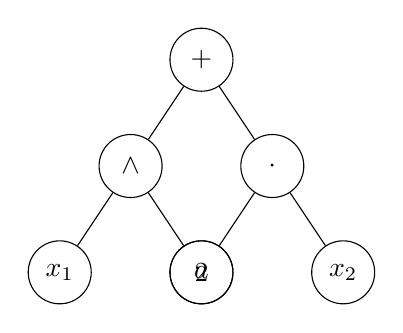
\begin{tikzpicture}[scale=0.9, every node/.style={draw, circle, minimum size=8mm, inner sep=0pt}, level distance=1.5cm, sibling distance=2cm]
        \node {$+$} child { node {$\wedge$} child { node {$x_1$} } child { node {$2$} } } child { node {$\cdot$} child { node {$a$} } child { node {$x_2$} } };
    \end{tikzpicture}
    \caption{Árbol sintáctico de la expresión $x_1^2 + a \cdot x_2$.} \label{fig:arbol_sintactico}
\end{figure}

La programación genética trabaja con una población de individuos (árboles) que se modifica a lo largo de generaciones —ciclos iterativos del proceso evolutivo— mediante los siguientes operadores:

\begin{itemize}
    \item \textbf{Selección}: Los individuos que producen predicciones más cercanas a los valores reales tienen mayor probabilidad de pasar a la siguiente generación.

    \item \textbf{Cruce}: Dos árboles padres intercambian subárboles para generar descendientes que combinan características de ambos.

    \item \textbf{Mutación}: Se reemplaza aleatoriamente un nodo o subárbol por otro nuevo, introduciendo diversidad en la población.

    \item \textbf{Elitismo}: Una fracción de los mejores individuos de cada generación se preserva sin cambios en la siguiente, evitando así que se pierdan las soluciones más prometedoras. Este mecanismo es opcional y su intensidad depende del problema \cite{koza1992genetic}.
\end{itemize}

La repetición de estos operadores a lo largo de las generaciones permite explorar el espacio de posibles expresiones algebraicas, guiando la búsqueda hacia funciones que se ajustan cada vez mejor a los datos \cite{koza1992genetic}.

La calidad de cada individuo se mide mediante una función de pérdida, cuyas variantes más relevantes para este trabajo se presentan a continuación.

\subsection{Funciones de pérdida}

La \textbf{función de pérdida} ---también llamada función de aptitud en el contexto de los algoritmos evolutivos--- es el criterio que se utiliza para evaluar cuantitativamente qué tan buena es una expresión candidata producida por la regresión simbólica. Esta función mide la discrepancia entre las predicciones de la expresión simbólica y los valores observados en el conjunto de datos. Una función de pérdida común, y la que se emplea como referencia en este trabajo, es el error cuadrático medio.

\textbf{Error cuadrático medio.} Para un conjunto de datos \(\{(\mathbf{u}_i, v_i)\}_{i=1}^{N}\) con \(\mathbf{u}_i \in \R^d\) y \(v_i \in \R\), y una función \(f: \R^d \to \R\), el error cuadrático medio (MSE, por sus siglas en inglés) se define como \begin{equation} \text{MSE}(f) = \frac{1}{N} \sum_{i=1}^{N} \left( v_i - f(\mathbf{u}_i) \right)^2, \end{equation} donde: \begin{itemize} \item \(N\) es el número total de puntos en el conjunto de datos, \item \(v_i\) es el valor observado para el \(i\)-ésimo punto, \item \(f(\mathbf{u}_i)\) es el valor predicho por la expresión \(f\) para el vector de entrada \(\mathbf{u}_i\). \end{itemize} El MSE penaliza cuadráticamente las desviaciones, por lo que es sensible a valores atípicos \cite{hastie2009elements}. En el contexto de la regresión simbólica, es una de las funciones de pérdida más utilizadas debido a su simplicidad y a que proporciona una señal suave para guiar el proceso de búsqueda \cite{bishop2006pattern}.

La efectividad del proceso evolutivo no solo depende de la función de pérdida elegida, sino también de la configuración del algoritmo. A continuación se describen los parámetros que controlan el comportamiento de la programación genética aplicada a la regresión simbólica.

\subsection{Parámetros del algoritmo de regresión simbólica}

El comportamiento de la regresión simbólica basada en programación genética depende de un conjunto de parámetros que influyen en la calidad de las soluciones, el tiempo de cómputo y la interpretabilidad de los resultados \cite{cranmer2023pysr}. A continuación se describen los más relevantes, agrupados según el aspecto del algoritmo que controlan.

\medskip \noindent\textbf{Parámetros de la población.}
\begin{itemize}
    \item \textbf{Tamaño de la población} (\(P\)): Número de individuos que coexisten en cada generación. Una población grande aumenta la diversidad genética y la probabilidad de encontrar soluciones de alta calidad, a cambio de un mayor tiempo de cómputo y consumo de memoria.

    \item \textbf{Número de generaciones} (\(G\)): Cantidad máxima de iteraciones. Un número elevado permite explorar más a fondo el espacio de búsqueda, aunque también incrementa el costo computacional.

    \item \textbf{Número de poblaciones independientes}: En algunas implementaciones se utiliza un modelo de islas, que consiste en dividir la población total en varias subpoblaciones que evolucionan en paralelo. Periódicamente, un pequeño número de individuos migra entre las islas, lo que ayuda a mantener la diversidad genética y evita la convergencia prematura \cite{whitley1990island}.
\end{itemize}

\medskip \noindent\textbf{Parámetros de control de la complejidad.} Además de la precisión, interesa obtener expresiones sencillas que sean fáciles de interpretar. Los siguientes parámetros regulan el equilibrio entre ajuste a los datos y simplicidad de las fórmulas.

\begin{itemize}
    \item \textbf{Coeficiente de parsimonia} (\(\alpha\)): Penalización añadida a la función de pérdida, proporcional al tamaño del árbol (número de nodos). La pérdida efectiva se calcula como
          \[
          \mathcal{L}_{\text{eff}}(f) = \text{MSE}(f) + \alpha \cdot \text{tamaño}(f).
          \]
          Un valor mayor de \(\alpha\) favorece expresiones más simples.

    \item \textbf{Tamaño máximo del árbol} (\(S_{\max}\)): Límite en el número de nodos que puede tener un individuo. Evita la explosión de la complejidad y reduce el espacio de búsqueda.
\end{itemize}

\medskip \noindent\textbf{Probabilidades de operadores genéticos.} La composición de cada nueva generación está determinada por las siguientes probabilidades, que deciden qué operador se aplica a cada individuo.

\begin{itemize}
    \item \textbf{Probabilidad de cruce} (\(p_c\)): Fracción de la nueva generación generada mediante cruce de padres seleccionados.

    \item \textbf{Probabilidad de mutación} (\(p_m\)): Fracción de individuos creados mediante modificaciones aleatorias de los árboles existentes.

    \item \textbf{Probabilidad de reproducción} (\(p_r\)): Fracción de individuos que pasan directamente a la siguiente generación sin cambios (elitismo), con \(p_r = 1 - p_c - p_m\).
\end{itemize}

El proceso completo funciona de la siguiente manera: se genera una población inicial de árboles aleatorios, cada árbol se evalúa con la función de pérdida y se seleccionan los mejores para la siguiente generación. Mediante cruce y mutación se crean nuevos individuos, mientras que el elitismo preserva las mejores soluciones. Este ciclo se repite durante un número prefijado de generaciones o hasta que se alcanza una calidad suficiente, dando como resultado una expresión analítica que aproxima los datos.

Para analizar estadísticamente los resultados obtenidos con este proceso, en el capítulo de experimentación se emplea la prueba t pareada, cuyos fundamentos se presentan a continuación.

\section{Prueba t pareada}
\label{sec:prueba_t}

En el Capítulo~\ref{sec:experimentacion} se comparan distintas funciones de pérdida evaluadas sobre los mismos casos de prueba. Para determinar si una de ellas ofrece un desempeño significativamente mejor que otra se utiliza la \textit{prueba t de Student para muestras pareadas} \cite{montgomery2017applied}. Esta prueba contrasta la hipótesis nula frente a la hipótesis alternativa, que se formulan como
\[
H_0 : \mu_d = 0 \qquad\text{frente a}\qquad H_1 : \mu_d > 0 \quad\text{o}\quad H_1 : \mu_d < 0,
\]
donde \(\mu_d\) es la media de las diferencias entre los dos métodos. La dirección de la desigualdad en \(H_1\) depende de si se quiere probar que un método supera al otro (en tasa de éxito) o que es más rápido (en tiempo de ejecución).

Si se denota por \(d_i = x_i - y_i\) la diferencia entre los resultados de dos métodos para el \(i\)-ésimo caso, el estadístico de prueba se calcula como
\[
t = \frac{\bar{d}}{s_d / \sqrt{n}}\,, \qquad \bar{d} = \frac{1}{n}\sum_{i=1}^{n} d_i\,,\; s_d = \sqrt{\frac{1}{n-1}\sum_{i=1}^{n} (d_i - \bar{d})^2}\,,
\]
donde \(n\) es el número de pares.

Bajo el supuesto de que las diferencias \(d_i\) son independientes y provienen de una población aproximadamente normal —condición que puede verificarse mediante una prueba de normalidad como la de Shapiro-Wilk—, el estadístico \(t\) sigue una distribución \(t\) de Student con \(n-1\) grados de libertad \cite{montgomery2017applied}. Esta distribución es simétrica y con colas más pesadas que la distribución normal estándar, especialmente para tamaños muestrales pequeños. El parámetro que determina su forma es el número de grados de libertad, \(\nu = n-1\), que refleja la cantidad de datos disponibles para estimar la variabilidad de las diferencias. Conforme
\(\nu\) crece, la distribución \(t\) se aproxima a la normal.

A partir del valor observado de \(t\) y de los grados de libertad se obtiene el \(p\)-valor, que indica la probabilidad de obtener un resultado al menos tan extremo como el observado si la hipótesis nula fuera cierta. Fijado un nivel de significación \(\alpha = 0.05\), la decisión se toma comparando el estadístico \(t\) con el valor crítico
\(t_{\alpha, \nu}\) que deja una probabilidad \(\alpha\) en la cola
correspondiente de la distribución \(t\) de Student. Si la hipótesis alternativa es \(H_1 : \mu_d > 0\), se rechaza \(H_0\) cuando
\(t > t_{\alpha, \nu}\); si la alternativa es \(H_1 : \mu_d < 0\), se
rechaza \(H_0\) cuando \(t < -t_{\alpha, \nu}\). Equivalentemente, se rechaza \(H_0\) si el \(p\)-valor es menor que \(\alpha\).

En los análisis del Capítulo~\ref{sec:experimentacion} se aplica la prueba t pareada para comparar tanto la tasa de éxito como el tiempo de ejecución de las distintas funciones de pérdida, indicando en cada caso el valor del estadístico \(t\) y el correspondiente \(p\)-valor.

Con los fundamentos presentados en este capítulo —sistemas no lineales, métodos numéricos, regresión simbólica y prueba t pareada— se cuenta con las herramientas necesarias para desarrollar la metodología que se presenta en el capítulo siguiente.